\documentclass[12pt]{standalone}
\usepackage{fontspec}
\setsansfont{TeX Gyre Heros}
\newfontfamily\mfallback{DejaVu Sans}
\usepackage{tikz}
\usetikzlibrary{arrows.meta}
\usepackage{amsmath}
\begin{document}
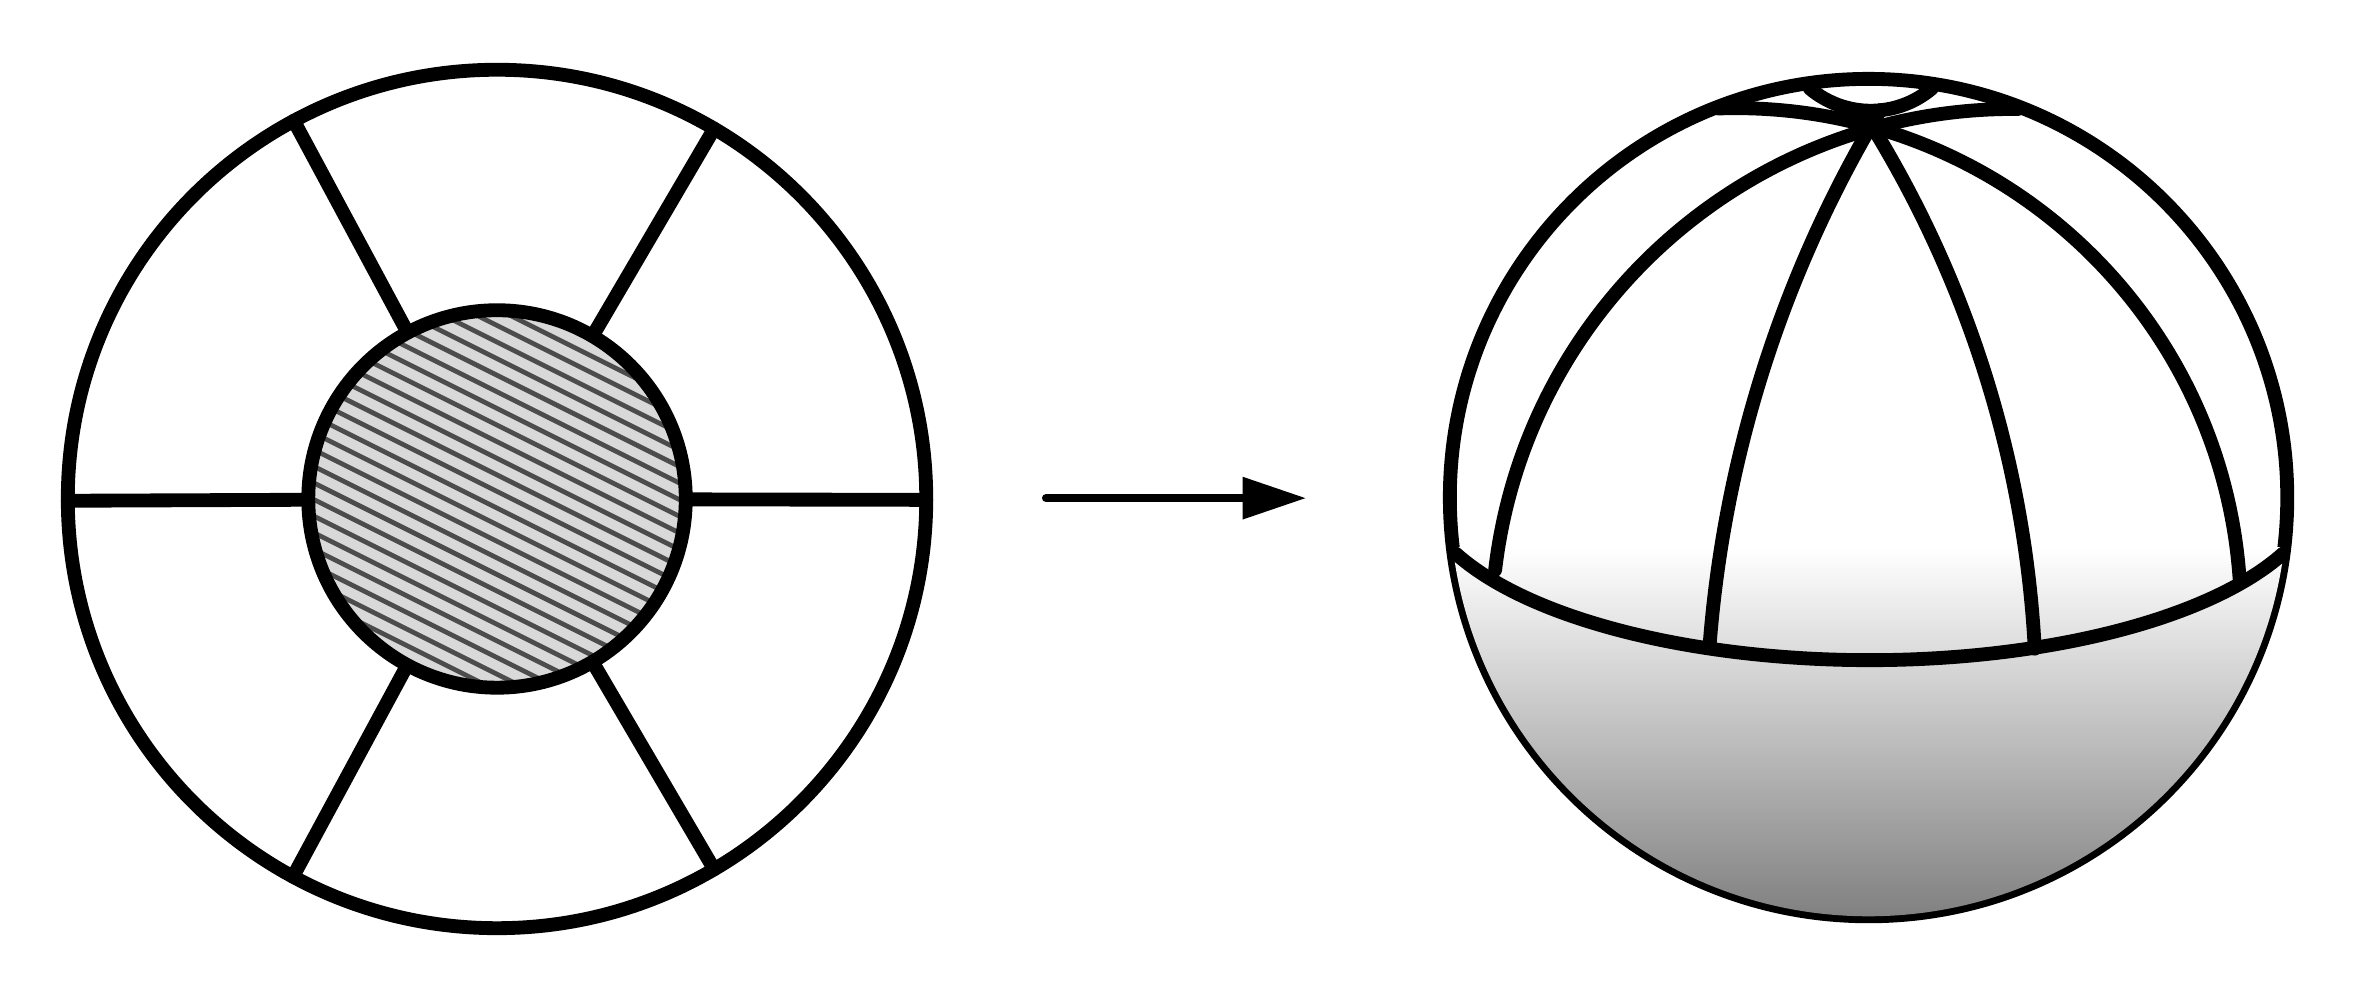
\begin{tikzpicture}[x=1pt, y=-1pt, line cap=round, line join=round, line width=5pt]

  % ==================== 左：圆盘（外套圆 + 实心内盘 + 6 条辐线）====================
  % 外套圆：骨架圆拟合 (169.2,170.3) r=155.0（横 153.4 / 竖 157.1，1.4% 扫描误差 -> circle）
  \draw (169.6,170.3) circle (155.1);

  % 6 条辐线：一条视觉元素一条命令；角度按墨迹射线量测
  \draw (169.6,170.3) ++(0.12:68.2)   -- ++(0.12:86.9);
  \draw (169.6,170.3) ++(59.62:68.2)  -- ++(59.62:86.9);
  \draw (169.6,170.3) ++(118.38:68.2) -- ++(118.38:86.9);
  \draw (169.6,170.3) ++(179.76:68.2) -- ++(179.76:86.9);
  \draw (169.6,170.3) ++(241.75:68.2) -- ++(241.75:86.9);
  \draw (169.6,170.3) ++(300.38:68.2) -- ++(300.38:86.9);

  % 实心内圆盘：中心量测 (170.0,170.3)，半径 68.2（600dpi 核为实心，非空环）
  %% 内圆盘：45 度排线（受光面，不是实心黑）
  \begin{scope}
    \clip (169.6,170.3) circle (68.2);
    \fill[black!15] (169.6,170.3) circle (68.2);
    \foreach \b in {-130,-124,...,130}
      \draw[black!70,line width=1.7pt] (95,{170.3+\b}) -- (245,{170.3+\b+75});
  \end{scope}
  \draw (169.6,170.3) circle (68.2);

  % ==================== 中间箭头 ====================
  % 杆 y=170（x 368..439，粗 3px），头基 x=439 高 15，尖 x=462
  \draw[line width=3pt, -{Triangle[length=23pt,width=14.6pt]}] (368,170) -- (462,170);

  % ==================== 右：球面 ====================
  % 球轮廓：骨架圆拟合 (665.6,167.5) r=149.6 与四点口径折中 -> (665.2,169.8) r=151.3；
  % 底缘竖向量到 154.5 是重印+阴影并线（1.6%），按球体规则用 circle
  \draw (665.2,169.8) circle (151.3);

    % 下缘阴影：球下半部浅灰渐变
  \begin{scope}
    \clip (665.2,169.8) circle (151.3);
    \shade[top color=white, bottom color=black!50]
      (514,188) rectangle (816,322);
  \end{scope}

  % 顶部小环（坍缩后的边界圆）：只画前/下半弧（上半被球轮廓压住）
  % 弧过 (644,22)-(666,30)-(688,22)：R=(22^2+8^2)/(2*8)=34.25，圆心 (666,-4.25)
  \draw (644.0,22.0) arc[start angle=130.0, end angle=50.0, radius=34.25];

  % 4 条内部经线：最小二乘圆拟合残差 0.2~0.3px -> 一律 arc
  % M1 左外：圆心 (717.6,218.0) r=188.63；端点沿极点的水平切线延伸到球轮廓（原书 x≈720）
  \draw (530.26,195.99) arc[start angle=-173.3, end angle=-89.5, radius=188.63];
  % M2 左内：圆心 (1048.01,257.18) r=441.57
  \draw (607.68,224.10) arc[start angle=-175.7, end angle=-149.0, radius=441.57];
  % M3 右内：圆心 (325.17,245.42) r=400.63
  \draw (725.25,224.39) arc[start angle=-3.01, end angle=-32.5, radius=400.63];
  % M4 右外：圆心 (617.21,211.58) r=182.48；端点沿极点的水平切线延伸到球轮廓（原书 x≈611）
  \draw (799.26,199.00) arc[start angle=-3.95, end angle=-92.0, radius=182.48];

  % 下部纬线弧（内圆盘的像）：椭圆中心 (665.5,163.9)，半轴 163.4 / 64.6；
  % 与球轮廓交于 (516.0,190.0)、(815.0,190.0)，下探至 (666,228.5)
  \draw (516.0,190.0) arc[start angle=156.2, end angle=23.8, x radius=163.4, y radius=64.6];

  % 钉死画布：1px = 1pt
  \pgfresetboundingbox
  \path[use as bounding box] (0,0) rectangle (831,342);
\end{tikzpicture}
\end{document}
